\hypertarget{a00848}{}\section{Example Plug-\/\+Ins}
\label{a00848}\index{Example Plug-\/Ins@{Example Plug-\/Ins}}
Descriptions of the S\+DK\textquotesingle{}s example plug-\/ins. 

\hypertarget{a00848_examples}{}\subsection{S\+D\+K Example plug-\/ins}\label{a00848_examples}
This S\+DK includes the following example plug-\/ins. These plug-\/ins are designed to demonstrate good A\+AX plug-\/in design with varying levels of complexity.

In general, the S\+DK includes one basic version of each example plug-\/in, as well as multiple variations on this basic version. Each of these variations demonstrates a particular feature or design approach. To see the specific changes that were made to implement a feature, compare the example plug-\/in variant that demonstrates the feature to the basic version of the plug-\/in.

Aside from the G\+UI Extension examples, which are designed to work with third-\/party G\+UI frameworks, each sample plug-\/in should successfully compile \char`\"{}out of the box\char`\"{}. However, you may receive compilation errors during the plug-\/ins\textquotesingle{} post-\/build copy step due to the fact that compiled TI D\+L\+Ls are not included with this S\+DK.\hypertarget{a00848_basic_examples}{}\subsubsection{Basic examples}\label{a00848_basic_examples}
These plug-\/ins provide complete working examples of A\+AX plug-\/ins without a lot of extra features. Use these plug-\/ins as a starting point for understanding \mbox{\hyperlink{a00852}{A\+AX}}.\hypertarget{a00848_DemoGain}{}\paragraph{Demo\+Gain}\label{a00848_DemoGain}
Demo\+Gain is the simplest example plug-\/in, incorporating a mono algorithm with gain and bypass parameters.\hypertarget{a00848_DemoDist}{}\paragraph{Demo\+Dist}\label{a00848_DemoDist}
Demo\+Dist demonstrates some more sophisticated techniques such as coefficient calculation and packaging, private data allocation, and multiple stem format support. Demo\+Dist also demonstrates some basic optimization strategies for improving real-\/time algorithmic performance.\hypertarget{a00848_DemoDelay}{}\paragraph{Demo\+Delay}\label{a00848_DemoDelay}
Demo\+Delay implements a basic delay algorithm. The variants of this example demonstrate a variety of alternative processing features provided by \mbox{\hyperlink{a00852}{A\+AX}}.\hypertarget{a00848_DemoMIDI_NoteOn}{}\paragraph{Demo\+M\+I\+D\+I\+\_\+\+Note\+On}\label{a00848_DemoMIDI_NoteOn}
Demo\+M\+I\+D\+I\+\_\+\+Note on demonstrates basic M\+I\+DI input functionality. The example will create a step function with every Note On and Note Off message it receives. It also shows how to handle M\+I\+DI packages in the Data Model by overriding the \mbox{\hyperlink{a01481_aac6fa72278c0f46aa430cd79bdb2d767}{A\+A\+X\+\_\+\+C\+Effect\+Parameters\+::\+Update\+M\+I\+D\+I\+Nodes()}} method.\hypertarget{a00848_RectiFi}{}\paragraph{Recti\+Fi}\label{a00848_RectiFi}
This is a fully ported version of the Recti-\/\+Fi plug-\/in from Avid\textquotesingle{}s D-\/\+Fi suite. For more information about Recti-\/\+Fi, see \href{http://www.avid.com/plugins/d-fi}{\texttt{ http\+://www.\+avid.\+com/plugins/d-\/fi}}

\begin{DoxyNote}{Note}
The S\+DK\textquotesingle{}s Recti-\/\+Fi example plug-\/in is currently out of date and does not accurately represent Avid\textquotesingle{}s shipping Recti-\/\+Fi plug-\/in.
\end{DoxyNote}
\hypertarget{a00848_feature_examples}{}\subsubsection{Feature examples}\label{a00848_feature_examples}
Each of these plug-\/ins is a slight variation on one of the \mbox{\hyperlink{a00848_basic_examples}{Basic examples}}. Each feature example plug-\/in demonstrates a specific feature or a possible alternative design approach for the plug-\/in. Compare these plug-\/ins with the corresponding basic example plug-\/in when you want to understand how a feature or design should be applied to your own A\+AX plug-\/ins.\hypertarget{a00848_DemoGain_GUIExtensions}{}\paragraph{Demo\+Gain\+\_\+\+G\+U\+I\+Extensions}\label{a00848_DemoGain_GUIExtensions}
These examples demonstrate the use of various native and third-\/party G\+UI frameworks with \mbox{\hyperlink{a00852}{A\+AX}}. The examples that use third-\/party frameworks are configured to link to static libraries that combine the S\+DK\textquotesingle{}s \mbox{\hyperlink{a00838}{G\+UI Extensions}} (located in /\+Extensions/\+G\+UI) and the applicable third-\/party G\+UI framework. These libraries are not included in the S\+DK, and you will need to install the applicable framework S\+DK before it will be possible to compile these example plug-\/ins.\hypertarget{a00848_DemoGain_LinkedParameters}{}\paragraph{Demo\+Gain\+\_\+\+Linked\+Parameters}\label{a00848_DemoGain_LinkedParameters}
This example demonstrates parameter linking. The plug-\/in is a stereo version of Demo\+Gain, with options to link the left and right channels in two different modes.\hypertarget{a00848_DemoGain_Smoothed}{}\paragraph{Demo\+Gain\+\_\+\+Smoothed}\label{a00848_DemoGain_Smoothed}
This example demonstrates efficient algorithmic coefficient smoothing using a slight variation on the basic Demo\+Gain plug-\/in algorithm.\hypertarget{a00848_DemoGain_Background}{}\paragraph{Demo\+Gain\+\_\+\+Background}\label{a00848_DemoGain_Background}
This example demonstrates a background routine for algorithm processing. This example also uses the A\+AX \mbox{\hyperlink{a00803}{direct data interface}} for communicating algorithmic delay to the plug-\/in\textquotesingle{}s controller.\hypertarget{a00848_DemoGain_DMA}{}\paragraph{Demo\+Gain\+\_\+\+D\+MA}\label{a00848_DemoGain_DMA}
This example includes two Effects that demonstrate use of the Scatter/\+Gather and Burst D\+MA facilities in \mbox{\hyperlink{a00852}{A\+AX}}.\hypertarget{a00848_DemoGain_Multichannel}{}\paragraph{Demo\+Gain\+\_\+\+Multichannel}\label{a00848_DemoGain_Multichannel}
This example demonstrates a multichannel plug-\/in configuration supporting all available point source stem formats.

This plug-\/in also includes a simple example of gain-\/reduction metering, which can be used to test host features which use this data such as the \mbox{\hyperlink{a00830_subsubsection__external_metering_and_internal_clip_}{gain reduction meters}} in Pro Tools.\hypertarget{a00848_DemoGain_UpMixer}{}\paragraph{Demo\+Gain\+\_\+\+Up\+Mixer}\label{a00848_DemoGain_UpMixer}
This example demonstrates conversion between different stem formats\hypertarget{a00848_DemoGain_ParamValueInfo}{}\paragraph{Demo\+Gain\+\_\+\+Param\+Value\+Info}\label{a00848_DemoGain_ParamValueInfo}
This example demonstrates an implementation of the \mbox{\hyperlink{a01669_a1702de6d62b5b41b6a8b2f510300392b}{Get\+Parameter\+Value\+Info()}} method, which is used to properly display certain parameter details on attached control surfaces. See \mbox{\hyperlink{a00833_aax_page_table_guide_04_avid_center_section_page_tables}{Avid Center Section Page Tables}} in the \mbox{\hyperlink{a00833}{Page Table Guide}}.\hypertarget{a00848_DemoDist_GenCoef}{}\paragraph{Demo\+Dist\+\_\+\+Gen\+Coef}\label{a00848_DemoDist_GenCoef}
This example demonstrates an alternative approach to parameter update handling. It bypasses the packet dispatcher helper class and directly overrides \mbox{\hyperlink{a01669_a685858711efb8634ce66c327f2865c71}{Update\+Parameter\+Normalized\+Value()}} and \mbox{\hyperlink{a01669_a083265b008921b6114ede387711694b7}{Generate\+Coefficients()}}. This approach may be appropriate for plug-\/ins that involve complex mapping between parameter updates, coefficient generation algorithms, and coefficient data packets.\hypertarget{a00848_DemoDelay_HostProcessor}{}\paragraph{Demo\+Delay\+\_\+\+Host\+Processor}\label{a00848_DemoDelay_HostProcessor}
This example includes two Effects that demonstrate the optional \mbox{\hyperlink{a00804}{Offline processing interface}} for advanced offline processing features. One Effect implements a simple offline delay line, while the other Effect implements the same delay line but compensates for its delay when rendering to the timeline. This demonstrates how to manually compensate for inherent algorithmic delay in an offline processor.

\begin{DoxyNote}{Note}
The output of offline plug-\/ins that do not use the \mbox{\hyperlink{a00804}{Offline processing interface}} will be automatically adjusted by the host host to account for any declared latency. The manual compensation technique demonstrated by Demo\+Delay\+\_\+\+Host\+Processor is {\bfseries{only}} necessary in plug-\/ins that implement the \mbox{\hyperlink{a00804}{Offline processing interface}}, e.\+g. plug-\/ins that require nonlinear offline processing features.
\end{DoxyNote}
\hypertarget{a00848_DemoDelay_Hybrid}{}\paragraph{Demo\+Delay\+\_\+\+Hybrid}\label{a00848_DemoDelay_Hybrid}
This example demonstrates the optional \mbox{\hyperlink{a00805}{Hybrid Processing architecture}} architecture for A\+AX plug-\/ins. This plug-\/in implements a short delay line that is rendered in the high-\/latency hybrid context. It can be built and run for either A\+AX Native or A\+AX D\+SP.\hypertarget{a00848_DemoDelay_DynamicLatencyComp}{}\paragraph{Demo\+Delay\+\_\+\+Dynamic\+Latency\+Comp}\label{a00848_DemoDelay_DynamicLatencyComp}
This example demonstrates how to properly handle algorithmic latency changes at run-\/time. It uses a delay line to emulate a latency-\/inducing algorithm with varying latency based on the delay parameter setting. When the plug-\/in\textquotesingle{}s latency compensation feature is enabled it declares this latency to the host.

\begin{DoxyRefDesc}{Host Compatibility Notes}
\item[\mbox{\hyperlink{a00786__compatibility_notes000011}{Host Compatibility Notes}}]The Demo\+Delay\+\_\+\+Dynamic\+Latency\+Comp example is compatible with Pro Tools 11.\+1 and higher.\end{DoxyRefDesc}
\hypertarget{a00848_DemoMIDI_Synth}{}\paragraph{Demo\+M\+I\+D\+I\+\_\+\+Synth}\label{a00848_DemoMIDI_Synth}
A basic synthesizer plug-\/in demonstrating use of an external object to manage the plug-\/in\textquotesingle{}s state. A\+AX Native plug-\/ins that are designed to work with a cross-\/format framework may use a similar design. This plug-\/in uses \mbox{\hyperlink{a01969}{A\+A\+X\+\_\+\+C\+Monolithic\+Parameters}} and therefore is A\+AX Native only.\hypertarget{a00848_DemoMIDI_Synth_AuxOutput}{}\paragraph{Demo\+M\+I\+D\+I\+\_\+\+Synth\+\_\+\+Aux\+Output}\label{a00848_DemoMIDI_Synth_AuxOutput}
A variation on \mbox{\hyperlink{a00848_DemoMIDI_Synth}{Demo\+M\+I\+D\+I\+\_\+\+Synth}} demonstrating the \mbox{\hyperlink{a00809}{Auxiliary Output Stems}} feature. This instrument plug-\/in supports four independently-\/routable synthesizer objects.\hypertarget{a00848_DemoMIDI_Sampler}{}\paragraph{Demo\+M\+I\+D\+I\+\_\+\+Sampler}\label{a00848_DemoMIDI_Sampler}
This simple \char`\"{}drum machine\char`\"{} style sampler plug-\/in demonstrates sample-\/accurate global and local M\+I\+DI input and the M\+I\+DI Transport interface. This plug-\/in uses \mbox{\hyperlink{a01969}{A\+A\+X\+\_\+\+C\+Monolithic\+Parameters}} and therefore is A\+AX Native only.\hypertarget{a00848_deprecated_examples}{}\subsubsection{Deprecated Examples}\label{a00848_deprecated_examples}
\hypertarget{a00848_DemoGain_Delay}{}\paragraph{Demo\+Gain\+\_\+\+Delay}\label{a00848_DemoGain_Delay}
\begin{DoxyRefDesc}{Deprecated}
\item[\mbox{\hyperlink{a00788__deprecated000001}{Deprecated}}]The Demo\+Gain\+\_\+\+Delay example is deprecated. See Demo\+Delay\+\_\+\+Host\+Processor\end{DoxyRefDesc}
Collaboration diagram for Example Plug-\/\+Ins\+:
\nopagebreak
\begin{figure}[H]
\begin{center}
\leavevmode
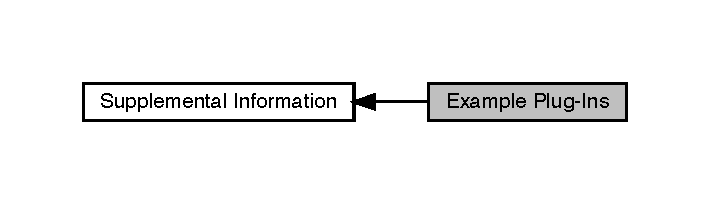
\includegraphics[width=340pt]{a00848}
\end{center}
\end{figure}
